
\documentclass[11pt]{beamer}
\usetheme{CambridgeUS}

\usepackage[utf8]{inputenc}
\usepackage[english]{babel}
\usepackage{amsmath}
\usepackage{amsfonts}
\usepackage{amssymb}
\usepackage{graphicx}
\usepackage{subfigure}
\usepackage{algorithm2e}
\usepackage{algorithmic}
\usepackage{url}
\usepackage{float}
\usepackage{xcolor}



% Puts the right page numbers for the presentation
\setbeamertemplate{footline}[frame number]

% Show uncovered items: 0 is invisible, 100 is fully visible
\setbeamercovered{transparent=3}

\author{Cody Eilar, Venkatesh Jatla, Mustafa Al-Mashhadani}
\title{Recommender Systems}
\logo{
\includegraphics[width=2.5cm]{figures/ecelogo.jpg}}
\institute{Dept of Electrical and Computer Engineering \\ The University of New Mexico \\ Albuquerque, NM 87131-0001, USA}
\date{\today}

\begin{document}
\maketitle

%--------------------- OUTLINE -------------------------%
\section{Outline}
\begin{frame}
  \frametitle{Outline}
  \begin{itemize}
    \item Collaborative filtering
      \begin{itemize}
        \item Overview
        \item Data normalization
        \item Validation block diagram
      \end{itemize}
    \item Content based filtering
      \begin{itemize}
        \item Block diagram
      \end{itemize}
  \end{itemize}
\end{frame}

%-------------------- COLLABORATIVE FILTERING ---------------%
\section{Collaborative filtering}
\begin{frame}
  \frametitle{Overview}
  \begin{figure}
    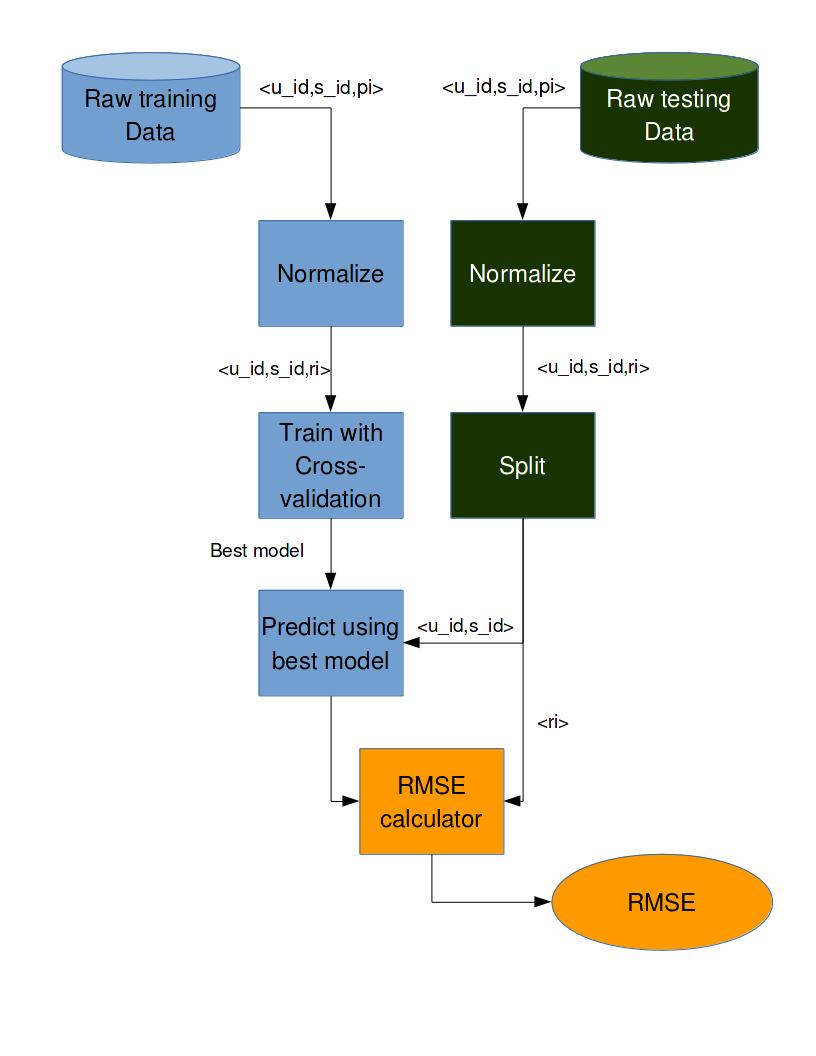
\includegraphics[width=0.5\linewidth]{figures/CollaborativeFilteringOverview.jpg}
  \end{figure}
\end{frame}

\begin{frame}
  \frametitle{Data normalization}
  \begin{itemize}
    \item Input Data = \{user\_id, song\_id, plays\}
    \item Normalize {\bf plays} so that
      \begin{itemize}
        \item 10 $=>$ Most liked song
        \item 0 $=>$ Most disliked song
      \end{itemize}
    \item If user $u_x$ has $P = \{p_1. p_2, p_3,\dots,p_n	\}$, then
      \begin{equation}
        r_i = 10 \times p_i/max\{P\}
      \end{equation}
  \end{itemize}
\end{frame}

\begin{frame}
  \frametitle{Validation block diagram}
  \begin{figure}
    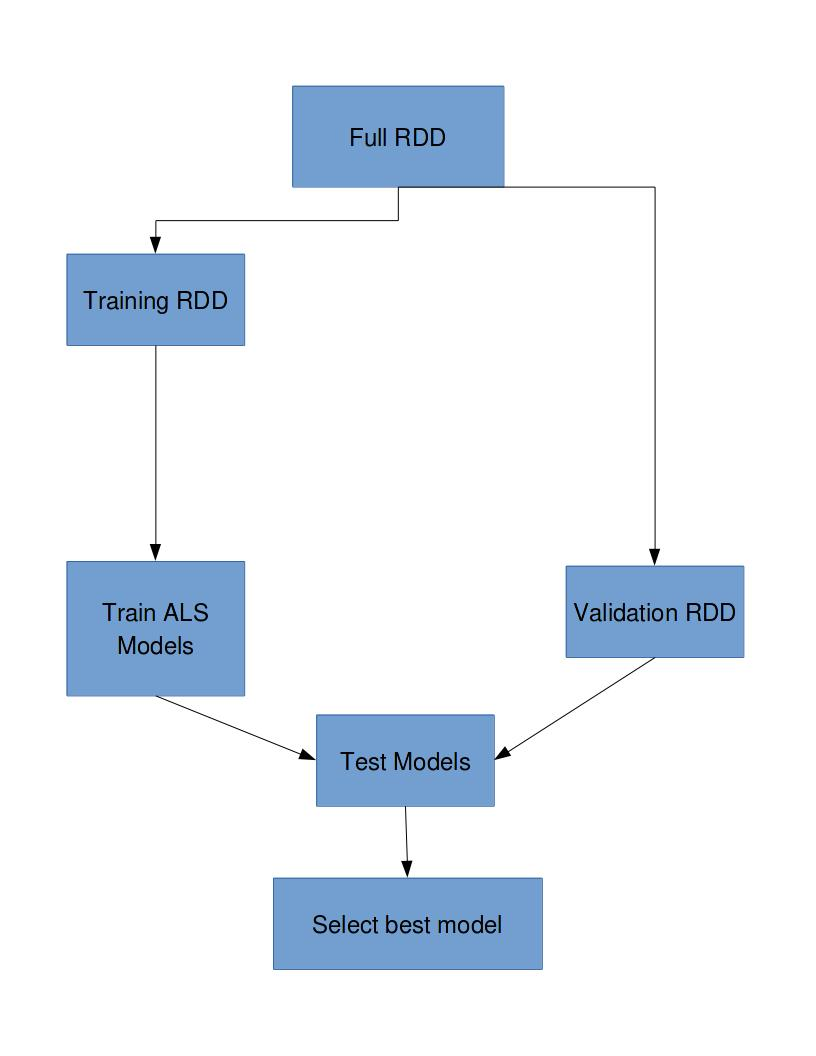
\includegraphics[width=0.5\linewidth]{figures/Validation.jpg}
  \end{figure}
\end{frame}

\begin{frame}
  \frametitle{Validation}
  \begin{itemize}
    \item Free parameters in ALS, \href{'http://spark.apache.org/docs/latest/mllib-collaborative-filtering.html'}{tutorial}
      \begin{itemize}
        \item rank, $\{R_0,R_1,\dots\}$
        \item lambda, $\{L_0,L_1,\dots\}$
        \item numIters, $\{N_0,N1,\dots\}$
      \end{itemize}
    \item Let input data RDD be, $R = \{row_i\}$, $row_i = \{user\_id_i, song\_id_i, r_i\}$
    \item Validation RDD is created by {\bf randomly sampling 10\%} of data RDD, $VS = 0.1R$
      \item Training RDD is creted by {\bf intersection compliment} of data RDD and Validation RDD,
        $TS = R - (R \cap VS)$
      \item Every possible combination is iterated and the model that gives {\bf minimum RMSE} on
        validation set, $VS$ is picked as best model.
    \end{itemize}
  \end{frame}

%--------------- CONTENT BASED FILTERING ------------------------%
  \section{Content Based Filtering}
  \begin{frame}
    \begin{figure}[!h]
      \frametitle{Block diagram}
      \centering
      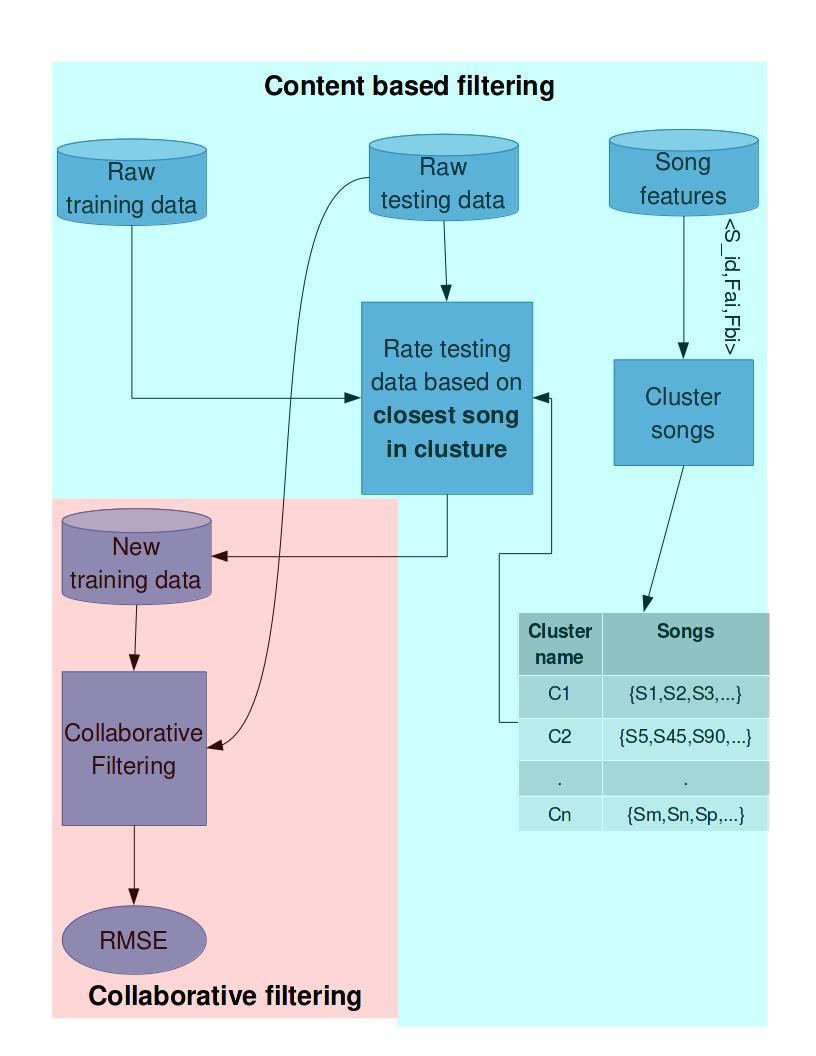
\includegraphics[width=0.5\linewidth]{figures/contentBasedBlockDiag.jpg}
      \caption{ Content enhanced collaborative filtering}
    \end{figure}
  \end{frame}

  \begin{frame}
    \frametitle{Features}
    For content based filtering we focused our effort on features that could be easily imported ({\it float values, almost all songs have them}). We found two such features,
    {\bf artist familiarity} and {\bf artist hotness}.
    \begin{table}
      \begin{tabular}{|p{4.5cm}|p{2cm} p{2cm} p{2cm}|}
        \hline
        {\bf song id} & {\bf familiarity} & {\bf hotness} & {\bf cluster id}\\
        \hline
        \hline
          SOQMMHC12AB0180CB8&           0.39&            0.64&       35\\
          SOVFVAK12A8C1350D9&           0.35&            0.43&       12\\
          SOGTUKN12AB017F4F1&           0.43&            0.64&        4\\
          SOBNYVR12A8C13558C&           0.37&            0.44&       12\\
          SOHSBXH12A8C13B0DF&           0.00&            0.00&       71\\
        \hline
      \end{tabular}
    \end{table}
  \end{frame}

  \begin{frame}
    \frametitle{Clustering}
    \begin{itemize}
      \item {\bf Method used:} K-means
      \item {\bf Number of clusters:} 100.
      \item {\bf Distance metric:} Euclidean distance.
      \item {\bf Running time:} 5 minutes
    \end{itemize}
  \end{frame}


%---------------- RESULTS and FUTURE WORK ---------------------%
  \section{Result and future work}
  \begin{frame}
    \frametitle{Results}
    \begin{table}
      \begin{tabular}{|p{5cm}|p{3cm} p{3cm}|}
        \hline
        {\bf Method} & {\bf RMSE} & {\bf Mean Absoute difference} \\
        \hline
        \hline
        {\color{red} Collaborative filtering} & {\color{red}$3.72$} & {\color{red}$2.63$}\\
        {\color{blue}Content enhanced collaborative filtering} & {\color{blue}$3.78$} & {\color{blue}$2.68$}\\
        \hline
      \end{tabular}
    \end{table}
  \end{frame}

  \begin{frame}
    \frametitle{Future Work}
    We observe that content based filtering is under performing. This might be fixed by,
    \begin{itemize}
      \item Increasing number of clusters beyond 100.
      \item Import extra features which may result in better clustering.
      \item Use a different metric in calculating distance.
    \end{itemize}
  \end{frame}

%--------------------- CODE BASE ------------------%
  \section{Code Base}
  \begin{frame}
    \begin{itemize}
      \item All code is here: https://github.com/AcidLeroy/MusicRecommender/
    \end{itemize}
  \end{frame}

%---------------------- QUESTIONS -------------------%
  \section{Questions?}
  \begin{frame}
    \frametitle{Questions?}

  \end{frame}


  \end{document}
